\documentclass[12pt,a4paper,violet,oneside]{bbe}
\usepackage{blindtext}
\usepackage{hyperref}
\usepackage{amsthm}
\usepackage{cleveref,extpfeil,extarrows}
\usepackage{algorithm, algorithmicx,algpseudocode}
\usepackage[version=4]{mhchem}
\usepackage{ctex}
\renewcommand{\algorithmicrequire}{\textbf{Input:}} 
\renewcommand{\algorithmicensure}{\textbf{Output:}}
%\input{zhwinfonts}
\begin{document}
\setcounter{chapter}{2}
\chapter{分治算法}
\section{分治算法简介}
本章我们正式进入对各类算法的学习,首先我们要介绍的是被称为\textbf{分治算法}的一类算法。

我们在程序设计思想与方法课程与数据结构课程中都经常接触一些在结构上是\textbf{递归的}算法,这些算法为解决一个问题,常常通过递归调用自身,解决一系列与原问题紧密相关的子问题以寻求原问题的解。从某种意义上来说,这类算法都遵循一种\textbf{分治}(\textbf{divide and conquer})的思想,以下,我们给出分治算法的具体定义:
\begin{definition}\label{def3.1}
	\textbf{分治算法}指这样一类算法:为解决原问题,将原问题分解为几个规模较小但类似于原问题的子问题,递归地求解这些子问题,然后再合并这些子问题的解来建立原问题的解。
\end{definition}

\hyperref[def3.1]{definition~3.1}给出了分治算法的定义,同时也给出了设计分治算法的\textbf{基本模式}:分治算法应当是\textbf{递归算法},且在每次递归中应包含以下\textbf{3}个步骤:
\begin{itemize}
	\item \textbf{分解}(\textbf{divide})原问题为若干子问题,这些子问题是原问题\textbf{规模较小的实例}。
	\item \textbf{解决}(\textbf{conquer})这些子问题,\textbf{递归}地求解这些子问题。然而,若子问题的规模足够小,则\textbf{直接求解}。
	\item \textbf{合并}(\textbf{merge})这些子问题的解形成原问题的解。
\end{itemize}

基于上述分析,我们可以对我们在递归算法复杂度分析中给出的分治算法复杂度$T(n)$满足的递推公式有进一步的理解:

$$
\left\{
\begin{array}{lcc}
	T(n)=aT(n/b)+f(n)&&n\geqslant2\\
	T(n)=c&&n=1\\
\end{array}\right.
$$


\begin{remark}
	此处我们不妨认为$T(n)$表示的是算法的\textbf{时间复杂度},且认为在之后的算法复杂度分析中关注的也主要为时间复杂度。
\end{remark}

在上式中,$T(n)=aT(n/b)+f(n)$代表将规模为$n$的原问题分解为$a$个规模为$n/b$的子问题,同时,对额外复杂度$f(n)$,可进一步分解为:
$$
f(n)=D(n)+C(n)
$$

其中$D(n)$为将原问题分解为子问题时引入的额外复杂度,$C(n)$为将子问题的解合并为原问题的解时所引入的额外复杂度。

以下,我们将通过一些具体的问题展示分治算法的设计与使用。
\section{分治算法示例1:归并排序}
\textbf{归并排序}(merge sort)是使用分治算法的一个最为经典,也最为简单的例子,其问题描述如\hyperref[ex3.1]{example~3.1}所示:

\begin{example}\label{ex3.1}
	给定规模为$n$的数组$A[1...n]$,设计算法将$A[1...n]$中的元素从小到大排序。
\end{example}

首先,我们按照分治算法“\textbf{分解-解决-合并}”的3个步骤初步确定算法设计的思路:首先应当分解原问题,这里很自然地一个想法就是将原数组$A[1...n]$的排序问题分解为两个子数组$A[1...p]$与$A[p+1...n]$的排序问题,不失一般性,我们可取这两个子数组在长度上“几乎”一致,即可取:
$$
p=\left\lfloor\frac{1+n}{2}\right\rfloor
$$

而我们可通过进一步递归调用原排序算法来解决$A[1...p]$与$A[p+1...n]$这两个子数组的排序问题,当然,若通过若干次递归后,需要进行排序的子数组\textbf{长度为1},则无需再进行分解,认为递归至此终止。

\begin{remark}
	虽然我们在分析问题时考虑了算法是如何一次次进行递归,直至递归终止的具体过程,但在实际算法设计时我们设计的其实只是进行每一次递归的一般化“\textbf{递归方式}”而非完整的“\textbf{递归过程}”,或者使用更为数学化的描述:我们给出的只是“\textbf{递推公式}”而非“\textbf{通项公式}”。对算法设计者而言,只需知道在递归终止条件设置正确且合理的情况下,递归地调用算法一定可以得出问题的解即可,而无需关心具体的递归求解过程。通过给出一般的递归方式以此来隐藏算法真正实现的冗杂流程,这也是递归算法的一个优势所在。
\end{remark}

而当我们通过递归调用原算法排序好$A[1...p]$与$A[p+1...n]$这两个子数组后,再将这两个排序好的数组合并为一个从小到大排序的有序数组即可。

其次,基于以上的分治算法设计,我们简单考虑一下这个算法的输入:一个平凡的输入为数组$A[1...n]$。另外,由于该算法的递归调用其实实现的是对数组$A[1...n]$中的若干连续子数组的排序,于是我们可以另加两个参数$p,r$,代表当前算法调用是用于排序数组$A[p...r]$。

因此,我们可给出如\cref{alo2.1}所示的\textbf{归并排序算法}:
\\
\begin{algorithm}[H]
	\caption{Merge Sort($A$,~$p$,~$r$)}
	\label{alo2.1}
	\begin{algorithmic}[1] 
		\Require 数组$A[1...n]$,待排序数组上界$r$,下界$p$
		\Ensure 元素从小到大排序的数组$A[p...r]$,对原问题仅需调用Merge Sort($A$,~$1$,~$n$) 
		\If {$p<r$}\textcolor{blue}{\Comment{当待排序的数组长度不小于2}}
		\State{$q=\lfloor(p+r)/2\rfloor$;}
		\State{Merge Sort($A$,~$p$,~$q$);}
		\State{Merge Sort($A$,~$q+1$,~$r$);}
		\State{Merge($A$,~$p$,~$q$,~$r$);}\textcolor{blue}{\Comment{对已完成排序的子数组进行\textbf{合并}}}
		\EndIf
		\State{\Return{$A[p...r]$};}
	\end{algorithmic} 
\end{algorithm}

在\cref{alo2.1}中,我们使用了一个函数Merge($A$,~$p$,~$q$,~$r$)对已排序完成的子数组$A[p...q]$与$A[q+1...r]$进行合并,最终得到的是排序完成的数组$A[p...r]$。以下我们考虑Merge($A$,~$p$,~$q$,~$r$)的具体实现:

Merge($A$,~$p$,~$q$,~$r$)实现的基本思路如下:将$A[p...q]$与$A[q+1...r]$视作两个栈,栈顶元素分别为$A[p]$与$A[q+1]$。首先,我们取$A[p]$与$A[q+1]$,即两个子数组的最小元素比较,则$\min\{A[p],~A[q+1]\}$必为$A[p...r]$中的最小元素,将该元素出栈,作为$A[p]$,再对两个栈顶元素进行比较,将较小者出栈并作为$A[p+1]$$\cdots$以此类推,当某一个栈空时,我们只需将非空栈的剩余元素按顺序出栈,顺次排列在已排序好的子数组后即可。

而为便于判断栈空,我们可以使用标准的栈结构对$A[p...q]$与$A[q+1...r]$进行存储,也可以简单地在$A[p...q]$与$A[q+1...r]$的末尾加入一个“\textbf{哨兵元素}”(此处我们取为$\infty$),当从子数组取出的元素为哨兵元素时,我们即认为该子数组已空。

基于此,我们给出的Merge($A$,~$p$,~$q$,~$r$)实现如\cref{alo2.2}所示:
\\
\begin{algorithm}[H]
	\caption{Merge($A$,~$p$,~$q$,~$r$)}
	\label{alo2.2}
	\begin{algorithmic}[1] 
		\Require 数组$A[1...n]$,子数组上/下界$p,~q,~r$
		\Ensure 元素从小到大排序的数组$A[p...r]$ 
		\State{$n_1=q-p+1$;}
		\State{$n_2=r-q$;}\textcolor{blue}{\Comment{计算$A[p...q]$与$A[q+1...r]$的长度}}
		\State{定义新数组$L[1...n_1+1]$与$R[1...n_2+1]$;}
		\State{$L[1...n_1]=A[p...q],~L[n_1+1]=\infty$;}
		\State{$R[1...n_2]=A[p+1...r],~R[n_2+1]=\infty$;}\textcolor{blue}{\Comment{子数组入栈,并定义哨兵元素}}
		\State{$i=j=1$;}
		\For{$k=p\to r$}
		\If{$L[i]\leqslant R[j]$}
		\State{$A[k]=L[i],~i=i+1$;}
		\ElsIf{$L[i]\geqslant R[j]$}
		\State{$A[k]=R[j],~j=j+1$;}
		\EndIf\textcolor{blue}{\Comment{由于$L[n_1+1]=R[n_2+1]=\infty$,因此不可能有元素比这两者大}}
		\EndFor
		\State{\Return{$A[p...r]$};}
	\end{algorithmic} 
\end{algorithm}

在解决问题后,我们来分析一下归并排序对应的时间复杂度:归并排序将一个规模为$n$的问题分解为$2$个规模为$n/2$的子问题,同时问题分解没有引入额外的时间复杂度,在使用Merge($A$,~$p$,~$q$,~$r$)对子问题的解进行合并时,对应的时间复杂度为$\Theta(n)$,于是有:
$$
T(n)=2T(n/2)+\Theta(n)
$$

利用主定理求解复杂度,得$T(n)=\Theta(n\log n)$,因此归并排序的时间复杂度为$\Theta(n\log n)$。
\section{分治算法示例2:逆序对}
\begin{example}
	假设$A[1...n]$是一个具有$n$个\textbf{互不相同}元素的数组,若无序对$(i,~j)$满足:
	$$
	i\ne j\wedge A[\min\{i,~j\}]>A[\max\{i,~j\}]
	$$
	
	则称$(i,~j)$为一个\textbf{逆序对},试确定$A[1...n]$中逆序对的数量。
\end{example}

对该问题,我们可采用与归并排序类似的思路设计算法:先将$A[1...n]$分解为两个子数组$A[1...p]$与$A[p+1...n]$,再分别递归地寻找$A[1...p]$与$A[p+1...n]$中的逆序对个数$r_L$与$r_R$,最后,寻找将$A[1...p]$与$A[p+1...n]$合并后的增加逆序对个数$r_M$,则总逆序对个数$r_0=r_L+r_R+r_M$,对应算法实现如\cref{alo2.3}所示:
\\
\begin{algorithm}[H]
	\caption{Count Inv($A$,~$p$,~$r$)}
	\label{alo2.3}
	\begin{algorithmic}[1] 
		\Require 数组$A[1...n]$,待操作数组上界$r$,下界$p$
		\Ensure  数组$A[p...r]$中的逆序对总数$r_0$,对原问题仅需调用Count Inv($A$,~$1$,~$n$)
		\If {$p<r$}\textcolor{blue}{\Comment{当待操作的数组长度不小于2}}
		\State{$q=\lfloor(p+r)/2\rfloor$;}
		\State{$r_L=$Count Inv($A$,~$p$,~$q$);}
		\State{$r_R=$Count Inv($A$,~$q+1$,~$r$);}
		\State{$r_M=$Merge Inv($A$,~$p$,~$q$,~$r$);}
		\EndIf
		\State{$r_0=r_L+r_R+r_M$;}\textcolor{blue}{\Comment{计算总逆序对个数}}
		\State{\Return{$r_0$};}
	\end{algorithmic} 
\end{algorithm}

在\cref{alo2.3}中我们同样使用了一个函数Merge Inv($A$,~$p$,~$q$,~$r$)来计算两个子数组合并后的增加的逆序对个数,以下,我们来讨论Merge Inv($A$,~$p$,~$q$,~$r$)的实现:

首先注意如下事实:\textbf{对子数组$A[p...q]$与$A[q+1...r]$而言,任意变动$A[p...q]$与$A[q+1...r]$内部的元素的顺序不会改变$A[p...q]$与$A[q+1...r]$合并后增加的逆序对个数。}这是一个较为显然的事实,因为对增加的逆序对$(i,~j)$,$A[i]$与$A[j]$一定是分属两个子数组的。

基于此,我们其实可以作如下断言:我们可以认为在调用Merge Inv($A$,~$p$,~$q$,~$r$)时,子数组$A[p...q]$与$A[q+1...r]$的内部元素是\textbf{有序排列}的。这是因为,我们完全可以使用Merge Inv($A$,~$p$,~$q$,~$r$)对子数组递归地进行排序,从而保证在调用Merge Inv($A$,~$p$,~$q$,~$r$)时,$A[p...q]$与$A[q+1...r]$就已经是有序的了。于是我们如\cref{alo2.4}所示实现Merge Inv($A$,~$p$,~$q$,~$r$):
\\
\begin{algorithm}[H]
	\caption{Merge Inv($A$,~$p$,~$q$,~$r$)}
	\label{alo2.4}
	\begin{algorithmic}[1] 
		\Require 数组$A[1...n]$,子数组上/下界$p,~q,~r$
		\Ensure $A[p...q]$与$A[q+1...r]$合并后增加的逆序对个数$r_M$ 
		\State{$n_1=q-p+1,~n_2=r-q$;}
		\State{$L[1...n_1]=A[p...q],~L[n_1+1]=\infty$;}
		\State{$R[1...n_2]=A[p+1...r],~R[n_2+1]=\infty$;}\textcolor{blue}{\Comment{子数组入栈,并定义哨兵元素}}
		\State{$i=j=1,~r_M=0$;}
		\For{$k=p\to r$}
		\If{$L[i]< R[j]$}
		\State{$A[k]=L[i],~i=i+1$;}
		\ElsIf{$L[i]> R[j]$}
		\State{$A[k]=R[j],~j=j+1,~r_M=r_M+(n_1-i+1)$;}\textcolor{blue}{\Comment{$L[i...n_1]$均与$R[j]$构成逆序对}}
		\EndIf
		\EndFor
		\State{\Return{$r_M$};}
	\end{algorithmic} 
\end{algorithm}
\begin{remark}
	有关$r_M=r_M+(n_1-i+1)$:存在另外一种写法是$r_M=r_M+j$,这种写法认为$L[i]>R[j]$代表$L[i]$与$R[1...j]$构成逆序对。这一说法本身是没问题的,但需要注意,若$L[i]>R[j]$,最终出栈的元素为$R[j]$,因此下一轮循环比较的是$L[i]$与$R[j+1]$,此时若$L[i]>R[j+1]$,则会重复计数$L[i]$与$R[1...j]$构成的逆序对,而原写法由于$R[j]$出栈,显然就不会在下一轮循环中导致重复。
\end{remark}
\begin{remark}
	有关为什么可以使用Merge Inv($A$,~$p$,~$q$,~$r$)对数组进行递归排序:回到\cref{alo2.1},仔细思考Merge Sort($A$,~$1$,~$n$)的递归过程,我们不难发现实际进行排序的其实是Merge($A$,~$p$,~$q$,~$r$),而我们递归地调用Merge Sort($A$,~$p$,~$r$)仅仅是为了确定Merge($A$,~$p$,~$q$,~$r$)的参数$p,~q,~r$。同样地,在Count Inv($A$,~$1$,~$n$)的调用过程中,实际对逆序对个数进行计数的也是Merge Inv($A$,~$p$,~$q$,~$r$),且递归调用Count Inv($A$,~$p$,~$r$)给出参数的过程与\cref{alo2.1}中完全相同。因此我们自然可以在Merge Inv($A$,~$p$,~$q$,~$r$)中嵌入对数组合并排序的过程。
	
	更具体一点说:在调用Merge Inv($A$,~$p$,~$q$,~$r$)前,必会先调用Merge Inv($A$,~$p$,~$\lfloor(p+q)/2\rfloor$,~$q$)与Merge Inv($A$,~$q+1$,~$\lfloor(q+1+r)/2\rfloor$,~$r$),这两次调用便会保证$A[p...q]$与$A[q+1...r]$的有序性,调用Merge Inv($A$,~$p$,~$q$,~$r$)后则会进一步保证$A[p..r]$的有序性。
\end{remark}

逆序对问题的分治算法的时间复杂度显然也是$\Theta(n\log n)$,如果单纯地遍历所有数对,再找出逆序对,则时间复杂度为$\Theta(n^2)$。
\section{分治算法示例3:大整数乘法}
\begin{example}
	给定两个\textbf{位数远大于}\textbf{机器字长}的$n$位大整数$X$与$Y$,计算$Z=X\cdot Y$。
\end{example}

针对这个问题,我们首先需要分析直接进行计算对应的时间复杂度,因为使用分治算法的根本目的就是简化计算的时间复杂度:传统的乘法需要先将$X$的每一位分别与$Y$相乘,再将结果相加,每一位相乘的时间复杂度均为$\Theta(n)$,乘法结果相加的时间复杂度也为$\Theta(n)$,进而总体的时间复杂度应为$\Theta(n^2)$,因此,一个理想的分治算法应当将计算的时间复杂度降至$\Theta(n^2)$以下。

但是,我们如果按传统的思路进行分治算法设计,记:
$$
X=A\cdot2^{\lfloor n/2\rfloor}+B,~Y=C\cdot2^{\lfloor n/2\rfloor}+D
$$

即将每个大整数分为高位部分与低位部分分别递归地进行计算,则:
$$
Z=X\cdot Y=AC\cdot2^{2\lfloor n/2\rfloor}+(AD+BC)\cdot2^{\lfloor n/2\rfloor}+BD
$$

可知对一个规模为$n$的乘法计算,最终可分解为$4$个规模为$n/2$的乘法计算,同时在合并时主要涉及\textbf{移位}与\textbf{求和}运算,会引入额外$\Theta(n)$的时间复杂度,因此时间复杂度$T(n)$满足的递推方程为:
$$
T(n)=4T(n/2)+\Theta(n)
$$

利用主定理求解,得$T(n)=\Theta(n^{\log_24})=\Theta(n^2)$,可知时间复杂度并没有得到简化。

而以下,我们将对上述的递归过程稍作改变,设计出一种能够有效提升计算效率的分治算法:

首先,我们仍采用相同的分治策略,记:
$$
X=A\cdot2^{\lfloor n/2\rfloor}+B,~Y=C\cdot2^{\lfloor n/2\rfloor}+D
$$

而我们注意到:
$$
\begin{array}{rl}
	Z&=X\cdot Y=AC\cdot2^{2\lfloor n/2\rfloor}+(AD+BC)\cdot2^{\lfloor n/2\rfloor}+BD\\
	&=AC\cdot2^{2\lfloor n/2\rfloor}+(AD+BC+AC+BD-AC-BD)\cdot2^{\lfloor n/2\rfloor}+BD\\
	&=AC\cdot2^{2\lfloor n/2\rfloor}+((A-B)(D-C)+AC+BD)\cdot2^{\lfloor n/2\rfloor}+BD
\end{array}
$$

于是,我们仅需计算$AC,~BD,~(A-B)(C-D)$这$3$个规模为$n/2$的乘法计算即可,而同时,分解与合并过程中所引入的额外时间复杂度仍为$\Theta(n)$。因此,采用这种分治算法对应时间复杂度的递推方程为:
$$
T(n)=3T(n/2)+\Theta(n)
$$

利用主定理求解,得$T(n)=\Theta(n^{\log_23})\approx\Theta(n^{1.59})$,可知这种分治算法可以有效提升计算效率。
\section{分治算法示例4:矩阵乘法的Strassen算法}
\begin{example}
	给定$n$阶方阵$A,~B$,计算$C=A\times B$。
\end{example}

为方便以下讨论,我们记:
$$
A=(a_{ij})_{n\times n},~B=(b_{ij})_{n\times n},~C=(c_{ij})_{n\times n}
$$

则对最传统的矩阵乘法而言,我们需要对每一个$c_{ij}$,计算:
$$
c_{ij}=\sum\limits_{k=1}^{n}a_{ik}b_{kj}
$$

对每一个$c_{ij}$,这样的\textbf{MAC运算}\footnote{Multiply Accumulate,乘累加运算}的时间复杂度均为$\Theta(n)$\footnote{这里将一次数字乘法与一次数字求和均作为一次基本操作,与大整数乘法不同,大整数乘法由于讨论的就是乘法这种运算的复杂度,因此是将计算机内部对二进制数码的一次操作视为一次基本操作},而这样的MAC运算需进行$n^2$次,因此总的时间复杂度为$\Theta(n^3)$。

而当我们尝试使用分治算法进行算法设计时,对原问题的分解思路其实也是比较平凡的,我们可以尝试利用分块矩阵对$A,~B$进行分解,记:
$$
A=\left[\begin{array}{cc}
	A_{11}&A_{12}\\
	A_{21}&A_{22}
\end{array}\right],~B=\left[\begin{array}{cc}
B_{11}&B_{12}\\
B_{21}&B_{22}
\end{array}\right]
$$

其中不妨记$A_{ij}$与$B_{ij}$均为$n/2$阶方阵\footnote{近似记法,此处的$n/2$也应解释为$\lfloor n/2\rfloor$或$\lceil n/2\rceil$}。

但我们如果仅局限于直接利用$C=A\times B$进行递归求解,则会发现:
$$
C=\left[\begin{array}{cc}
	C_{11}&C_{12}\\
	C_{21}&C_{22}
\end{array}\right]=\left[\begin{array}{cc}
	A_{11}&A_{12}\\
	A_{21}&A_{22}
\end{array}\right]\times\left[\begin{array}{cc}
	B_{11}&B_{12}\\
	B_{21}&B_{22}
\end{array}\right]
$$

最终会将规模为$n$的原问题分解为$8$个规模为$n/2$的子问题进行求解,而分解与合并过程中所引入的额外时间复杂度为$\Theta(n^2)$(由于涉及矩阵的相加),因此对应的时间复杂度$T(n)$满足递推方程:
$$
T(n)=8T(n/2)+\Theta(n^2)
$$

利用主定理求解,得$T(n)=\Theta(n^{\log_28})=\Theta(n^3)$。

因此,如大整数乘法一样,标准的分治策略无法简化计算的时间复杂度,我们需要在分块矩阵乘法的计算上进行进一步的改进。这里我们给出\textbf{Strassen}提出的一种分治策略,其对应实现的分治算法又被称为\textbf{Strassen算法}。

Strassen算法的一个特点在于:现阶段还很难直观地解释为什么要按照这样的思路设计分治策略,我们所能做的,仅仅是从数学角度验证算法的正确性。因此,我们直接给出Strassen算法的具体实现:

首先,计算如下的10个矩阵$S_1\sim S_{10}$:
$$
\begin{array}{ccccc}
	S_1=B_{12}-B_{22}&S_2=A_{11}+A_{12}&S_3=A_{21}+A_{22}&S_4=B_{21}-B_{11}&S_5=A_{11}+A_{22}\\
	S_6=B_{11}+B_{22}&S_7=A_{12}-A_{22}&S_8=B_{21}-B_{22}&S_9=A_{11}-A_{21}&S_{10}=B_{11}+B_{12}
\end{array}
$$

其次,计算如下的7个矩阵$P_1\sim P_7$:
$$
\begin{array}{ccccc}
P_1=A_{11}\cdot S_1&P_2=S_2\cdot B_{22}&P_3=S_3\cdot B_{11}&P_4=A_{22}\cdot S_4&P_5=S_5\cdot S_6\\
&P_6=S_7\cdot S_8&&P_7=S_9\cdot S_{10}&
\end{array}
$$

进而$C=A\times B$可由以下分块矩阵给出:
$$
C=\left[\begin{array}{cc}
	C_{11}&C_{12}\\
	C_{21}&C_{22}
\end{array}\right]=\left[\begin{array}{cc}
	P_5+P_4-P_2+P_6&P_1+P_2\\
	P_3+P_4&P_5+P_1-P_3-P_7
\end{array}\right]
$$

该算法定义的10个矩阵$S_1\sim S_{10}$仅涉及$A_{ij}$与$B_{ij}$的加减运算,引入的额外时间复杂度为$\Theta(n^2)$,计算$P_1\sim P_7$相当于7个规模为$n/2$的子问题,利用$P_1\sim P_7$计算$C=A\times B$也仅涉及$P_i$的加减运算,引入的额外时间复杂度为$\Theta(n^2)$,因此Strassen算法的时间复杂度$T(n)$对应的递推方程为:
$$
T(n)=7T(n/2)+\Theta(n^2)
$$

利用主定理求解,得$T(n)=\Theta(n^{\log_27})\approx\Theta(n^{2.81})$,可知计算效率要优于先前给出的$\Theta(n^3)$。

\section{分治算法示例5:最近点对问题}
\begin{example}
	给定\textbf{二维Euclidean 空间}上$n$个点的集合$S=\{p_1,\cdots,p_n\}$,输出两个点$p_i,~p_j$,使得$p_i,~p_j$的距离最短。两点$p_i=(x_i,~y_i),~p_j=(x_j,~y_j)$间的距离$\text{dis}(p_i,~p_j)$被定义为:
	$$
	\text{dis}(p_i,~p_j)=\sqrt{(x_i-x_j)^2+(y_i-y_j)^2}
	$$
\end{example}

同样,我们先分析暴力求解对应的时间复杂度,暴力求解意味着计算出:
$$
\text{dis}(p_i,~p_j),~\forall i,j,~1\leqslant i\ne j\leqslant n
$$

再寻找$\min\{\text{dis}(p_i,~p_j)|1\leqslant i\ne j\leqslant n\}$,这一过程的时间复杂度为$\Theta(n^2)$,因此,一个有效的分治算法设计应当能够保证算法的时间复杂度优于$\Theta(n^2)$。

我们仍按照“\textbf{分解-解决-合并}”的步骤设计分治策略:

首先,对于分解,我们可以以点$p_i=(x_i,~y_i)$的横坐标$x_i$为依据,取$\{x_i\}_{i=1}^n$的中位数$m$,作直线$x=m$,并将$x_i\leqslant m$的点(以下简称\textbf{左侧}的点)与$x_i>m$的点(以下简称\textbf{右侧}的点)分开进行求解。这两个子问题的结果分别代表$x_i\leqslant m$的点中距离最短的点对与$x_i>m$的点中距离最短的点对。

其次,将$x_i\leqslant m$的点与$x_i>m$的点合并,寻找这样的点对中距离最小的点对:
$$
\min\{\text{dis}(p_i,p_j)|x_i\leqslant m,~x_j>m\}
$$

再将找到的\textbf{3个}距离最短的点对比较,所得距离最短者即为原问题的最终解。

对以上思路而言,原问题的分解与解决都是易于解决的,问题的关键仍在于如何将子问题合并为原问题,我们记合并引入的额外时间复杂度为$f(n)$,则原问题时间复杂度$T(n)$对应满足的递推方程为:
$$
T(n)=2T(n/2)+f(n)
$$

使用主定理我们可知,为使分治算法对应的时间复杂度优于$\Theta(n^2)$,我们必须使$f(n)$的时间复杂度优于$\Theta(n^2)$。

对$f(n)$的要求使得我们无法使用遍历求解:
$$
\min\{\text{dis}(p_i,p_j)|x_i\leqslant m,~x_j>m\}
$$

因为$\{\text{dis}(p_i,p_j)|x_i\leqslant m,~x_j>m\}$共包含$\frac{n}{2}\cdot\frac{n}{2}=\frac{n^2}{4}$个距离值,遍历比较的时间复杂度为$\Theta(n^2)$。

而以下,我们注意到,如果$d_M=\min\{\text{dis}(p_i,p_j)|x_i\leqslant m,~x_j>m\}$能够成为最终的最小距离,则我们记:
$$
d_L=\min\{\text{dis}(p_i,p_j)|x_i,x_j\leqslant m\},~d_R=\min\{\text{dis}(p_i,p_j)|x_i,x_j> m\}
$$

应当成立:
$$
d_M\leqslant \min\{d_L,~d_R\}
$$

换言之,我们在计算$d_M$时,只需要计算那些距离可能小于$\min\{d_L,~d_R\}$的左侧与右侧点间的距离,而无需遍历求解全部的$\text{dis}(p_i,p_j)$。而如何判断一个左侧的点$p_i$与一个右侧的点$p_j$间的距离是否可能小于$\min\{d_L,~d_R\}$呢?我们可以给出一个粗略的估计,对左侧的点$p_i=(x_i,y_i)$而言,与其距离小于$d=\min\{d_L,~d_R\}$只可能分布于\textbf{矩形区域}:
$$
D(p_i)=\{(x,y)|m<x\leqslant m+d,~y_i-d\leqslant y\leqslant y_i+d\}
$$

$D(p_i)$是一个$d\times 2d$的矩形区域,而如果我们按\cref{fig1}所示对$D(p_i)$进行划分,将其划分为\textbf{6个}$d/2\times 2d/3$的矩形区域,则事实上我们不难发现,每个矩形区域内\textbf{至多存在一个点},这是因为,若假设某矩形区域内存在$u,~v$两个点,则:
\begin{figure}[!htbp]
	\centering
	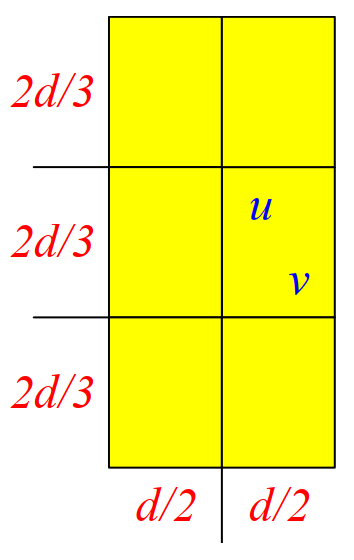
\includegraphics[width=4cm]{fig1}
	\caption{$D(p_i)$的划分}
	\label{fig1}
\end{figure}
$$
\text{dis}(u,v)\leqslant\sqrt{\left(\frac{2d}{3}\right)^2+\left(\frac{d}{2}\right)^2}<d
$$

这与$d=\min\{d_L,~d_R\}$矛盾!换言之,对左侧任意一点$p_i$,我们仅需对$D(p_i)$内存在的\textbf{至多6个点}进行考查,即可确定右侧是否存在点$p_j$,使得$\text{dis}(p_i,p_j)\leqslant \min\{d_L,~d_R\}$。

但此处存在一个的问题,我们应当如何判断右侧的点是否处于区域$D(p_i)$内呢?如果单纯按原问题中给出的无序点集逐个判断,则又会消耗$\Theta(n)$的时间复杂度,而对左侧的每个$p_i$都进行相同操作,对应的时间复杂度又变成了$\Theta(n^2)$。为此,我们可以在最开始就对无序点集\textbf{分别按$x$坐标与$y$坐标进行排序}(时间复杂度$\Theta(n\log n)$),这样判断右侧的点是否处于区域$D(p_i)$内可遵循以下步骤:
\begin{enumerate}
	\item 按\textbf{$y$坐标从小到大},找左侧$x$坐标介于$m-d\sim m$的点$p_i$与右侧$x$坐标介于$m\sim m+d$的点$p_j$\footnote{找到的$p_i,p_j$也自然地会按\textbf{$y$坐标从小到大}排序},只有这些$p_i,p_j$间的距离可能小于$d$。(时间复杂度$\Theta(n)$)
	\item 对找到的所有满足条件的左侧点$p_i$,按\textbf{$y$坐标从小到大}进行遍历,分别寻找位于$D(p_i)$内的右侧点$p_j$,这里的寻找方式是,假设满足条件的左侧点为($y$坐标从小到大):
	$$
	p^l_1,~p^l_2,\cdots,~p^l_s
	$$
	
	满足条件的右侧点为($y$坐标从小到大):
	$$
	p^r_1,~p^r_2,\cdots,~p^r_t
	$$
	
	则定义标识符$i,j$,初始值均为0。对$p^l_i,~i=1\to s$进行遍历,对每个$p^l_i$,记其$y$坐标为$y^l_i$,若$p^r_j$的$y$坐标$y^r_j$满足$y^r_j<y^l_i-d$,则$j\leftarrow j+1$,代表$p^r_j$不在$D(p^l_i)$中,自然也不可能在$D(p^l_k)$中($k>i$)\footnote{这里的$j$在对$p^l_i$的遍历过程中相当于一个\textbf{静态变量},在对$p^l_i$的遍历完成后不会被置0,而会保存当前的值进行下一个点$p^l_{i+1}$的遍历}。而当排除所有满足$y^r_j<y^l_i-d$的$p^r_j$后,定义一个新的标识符$u$\footnote{这里之所以要定义新标识符,是因为我们只能得到满足$y^r_j<y^l_i-d$的$p^r_j$不会在$D(p^l_k)$($k\geqslant i$)内,但不能判断$y^r_j\geqslant y^l_i-d$的$p^r_j$是否在$D(p^l_k)$($k\geqslant i$)内,因此在$p^l_{i+1}$的遍历过程中,$j$仍要从当前值开始计数,因而需要定义$u$来保护$j$的值不变},将其值置0,判断$p^r_{j+u}$是否满足$y^r_{j+u}\leqslant y^l_i+d$,若满足,则说明$p^r_{j+u}$在$D(p^l_i)$中,并计算$\text{dis}(p^l_i,p^r_{j+u})$,并比较与$d$的大小关系,而后令$u\leftarrow u+1$,进行下一个点的判断,直至$y^r_{j+u}>y^l_i+d$,结束对$p^l_i$的遍历,$i\leftarrow i+1$。(时间复杂度$\Theta(n)$\footnote{因为基本操作数由$j$与$u$进行计数,$j$最多计数$t$次,$u$对每个$i=1\to s$最多计数\textbf{6次},因此该程序的基本操作数不大于$t+6s$次,时间复杂度为$\Theta(n)$})
\end{enumerate}

综上,合并过程的时间复杂度为$\Theta(n)$,但同时\textbf{需引入对无序点集的排序}过程,从而增加$\Theta(n\log n)$的时间复杂度(\textbf{不在合并过程中,只是初始化处理}),进而可知算法整体的时间复杂度为$\Theta(n\log n)$。
\section{分治算法示例6:快速Fourier变换(FFT)}
\begin{example}
	已知\textbf{离散Fourier级数对}:
	$$
	a_k=\sum\limits_{n=<N>}x[n]\mathrm{e}^{-jk(2\pi/N)n}~(\text{正变换})
	$$
	$$
	x[n]=\frac{1}{N}\sum\limits_{k=<N>}a_k\mathrm{e}^{jk(2\pi/N)n}~(\text{逆变换})
	$$
	
	其中$k=<N>$指$k$取定$N$个连续整数,以下不妨记$k=0\to N-1$。
	
	现希望在已知序列$\{x[1],~x[2],\cdots,~x[N-1]\}$的情况下,求解序列$\{a_1,~a_2,\cdots,~a_{N-1}\}$,并且以下为方便讨论,我们不妨记\footnote{这里为何有“\textbf{不妨}”之说,我们之后会进行解释}$N=2^t$。
\end{example}

首先,不难发现,如果直接进行求解,则对规模为$N$的问题,共需要$N^2$次\textbf{复数乘法操作},如果我们将一次\textbf{乘法操作}记为一次基本操作,则直接计算的时间复杂度为$\Theta(n^2)$。以下,我们希望使用\textbf{分治算法}将计算的时间复杂度降至$\Theta(n\log n)$,为此,我们给出一种被称为\textbf{快速Fourier变换}(Fast Fourier Transform,~\textbf{FFT})的经典分治算法设计。

首先,为方便讨论,我们记$\omega_N=\mathrm{e}^{(2\pi/N)j}$,于是我们需要计算的Fourier正变换变为:
$$
a_k=\sum\limits_{n=0}^{N-1}x[n]\omega_N^{nk}
$$

对$n$分\textbf{奇偶}求和,同时注意$N=2^t$:
$$
a_k=\sum\limits_{m=0}^{N/2-1}x[2m]\omega_N^{(2m)k}+\sum\limits_{m=0}^{N/2-1}x[2m+1]\omega_N^{(2m+1)k}
$$

同时,我们显然有:$\omega_N^{2n}=\omega_{N/2}^{n}$,因此:
$$
a_k=\sum\limits_{m=0}^{N/2-1}x[2m]\omega_{N/2}^{mk}+\omega_N^{k}\sum\limits_{m=0}^{N/2-1}x[2m+1]\omega_{N/2}^{mk}
$$

为进一步简化,我们记$g[m]=x[2m],~h[m]=x[2m+1]$,则:
$$
a_k=\sum\limits_{m=0}^{N/2-1}g[m]\omega_{N/2}^{mk}+\omega_N^{k}\sum\limits_{m=0}^{N/2-1}h[m]\omega_{N/2}^{mk}=G_k+\omega_N^{k}H_k
$$

其中:
$$
G_k=\sum\limits_{m=0}^{N/2-1}g[m]\omega_{N/2}^{mk},~H_k=\sum\limits_{m=0}^{N/2-1}h[m]\omega_{N/2}^{mk}
$$

$\{G_k\}_{k=0}^{N/2-1}$与$\{H_k\}_{k=0}^{N/2-1}$分别为两个子序列$\{g[m]\}_{m=0}^{N/2-1}$与$\{h[m]\}_{m=0}^{N/2-1}$的Fourier正变换,但注意此处的$k$只能取$0\sim N/2-1$,因此对$0\leqslant k\leqslant N/2-1$的$a_k$,可以使用:
$$
a_k=G_k+\omega_N^{k}H_k
$$
进行计算,而对$N/2\leqslant k\leqslant N-1$的$a_k$,我们注意仍成立:
$$
a_k=\sum\limits_{m=0}^{N/2-1}g[m]\omega_{N/2}^{mk}+\omega_N^{k}\sum\limits_{m=0}^{N/2-1}h[m]\omega_{N/2}^{mk}
$$

进而我们记$k=l+N/2$,有$0\leqslant l\leqslant N/2-1$,且:
$$
a_{l+N/2}=\omega_{N/2}^{m(N/2)}\sum\limits_{m=0}^{N/2-1}g[m]\omega_{N/2}^{ml}+\omega_{N/2}^{m(N/2)}\cdot\omega_N^{k}\sum\limits_{m=0}^{N/2-1}h[m]\omega_{N/2}^{lk}
$$

注意$\omega_{M}^{M}=1$,则有:
$$
a_k=G_{k-N/2}+\omega_N^{k}H_{k-N/2}
$$

因此,我们得到了递归关系:
\begin{equation}
	\left\{\begin{array}{lcl}
		a_k=G_k+\omega_N^{k}H_k&&0\leqslant k\leqslant N/2-1\\
		
		a_k=G_{k-N/2}+\omega_N^{k}H_{k-N/2}&&N/2\leqslant k\leqslant N-1
	\end{array}\right.
\label{eq3.1}
\end{equation}

其中:$\{G_k\}_{k=0}^{N/2-1}$与$\{H_k\}_{k=0}^{N/2-1}$分别为$\{x[n]\}_{n=0}^{N-1}$的\textbf{偶子序列}与\textbf{奇子序列}的Fourier正变换。利用如\cref{eq3.1}所示的递归关系,我们即可设计如\cref{alo2.5}所示的\textbf{FFT算法}:
\\
\begin{algorithm}[H]
	\caption{FFT($x$,~$N$)}
	\label{alo2.5}
	\begin{algorithmic}[1] 
		\Require 数组$x[0...N-1]$及其长度$n$,$N=2^t$
		\Ensure  数组$x[0...N-1]$对应的Fourier正变换$a[0...N-1]$
		\State{$\omega_N=\mathrm{e}^{(2\pi/N)j}$;}
		\If {$N=2$}\textcolor{blue}{\Comment{当待变换的数组长度为2}}
		\State{$a[0]=x[0]+x[1],~a[1]=x[0]-x[1]$;}
		\State{\Return $a[0...N-1]$;}
		\EndIf
	\State{$G[0...N/2-1]\leftarrow$FFT($\{x[0],~x[2],\cdots,~x[N-2]\}$,~$N/2$);}
	\State{$H[0...N/2-1]\leftarrow$FFT($\{x[1],~x[3],\cdots,~x[N-1]\}$,~$N/2$);}
	\For{$k=0\to N/2-1$}
	\State{$a[k]\leftarrow G[k]+\omega_{N}^{k}H[k]$;}
	\State{$a[k+N/2]\leftarrow G[k]+\omega_{N}^{k+N/2}H[k]$;}\textcolor{blue}{\Comment{求解子数组的Fourier变换}}
	\EndFor
	\State{\Return $a[0...N-1]$;}
	\end{algorithmic} 
\end{algorithm}

不难发现,\cref{alo2.5}对应的FFT算法的时间复杂度为$\Theta(n\log n)$。

最后,我们讨论一下原题中对$N=2^t$的假设的合理性:对$N\ne 2^t$,我们事实上可设$2^{t-1}<N<2^t$,再令:
$$
x'[n]=\left\{\begin{array}{lcl}
	x[n]&&0\leqslant n\leqslant N-1\\
	0&&N\leqslant n\leqslant 2^t-1
\end{array}\right.
$$

这之后,对$\{x'[n]\}_{n=0}^{2^t-1}$应用FFT即可。但需要指出的是:一方面,对$\{x'[n]\}_{n=0}^{2^t-1}$进行Fourier变换的结果肯定\textbf{不同于}对$\{x[n]\}_{n=0}^{N-1}$进行Fourier变换的结果;另一方面,虽然两者不同,但基于\textbf{数字信号处理}的知识,这两者只是改变了频域采样的间隔,所反应的是同一个频谱$X(\mathrm{e^{j\omega}})$。
\section{分治算法示例7:剪枝搜索与线性时间选择算法}
\textbf{剪枝搜索}是用于进一步简化分治算法的一种方法,其主要指\textbf{利用计算问题特征,剪除不影响问题求解的输入数据,并利用剩下的输入数据构成与原问题形式相同,但规模更小的子问题,最后在子问题上递归调用算法求解问题}。

一般地,在使用剪枝搜索时我们希望剪枝时能剪除掉\textbf{常数因子}个输入数据(即对于规模为$n$的输入数据能够剪除$\lambda n$个输入数据,其中$\lambda$为与规模$n$无关的\textbf{常数因子}),而不是仅仅剪除个别数据。

以下,我们将以\textbf{选择问题}为例,简要讨论剪枝搜索的具体操作:
\begin{example}
	\textbf{选择问题}是指这样一类问题:
	
	\textbf{Input}:数组$A[1:n]$,正整数$k$,~$1\leqslant k\leqslant n$。
	
	\textbf{Output}:元素$A[i]\in A[1:n]$,使得$A[1:n]$中恰好有$k-1$个元素小于$A[i]$。
	
	换言之,选择问题其实就是在数组$A[1:n]$中寻找第$k$小元素的问题。
\end{example}

本节中我们使用剪枝搜索对该问题进行处理,使得最终设计的分治算法能够实现$O(n)$的时间复杂度(注意是$O(n)$,不是$\Theta(n)$)。

首先给出分治算法的基本设计思路,假设我们需要在数组$A[1:n]$中寻找第$k$小元素:
\begin{enumerate}
	\item 选择$A[1:n]$中的某个元素$A[m]$作为\textbf{划分点}。
	\item 利用$A[m]$对$A[1:n]$进行划分,划分得到三个集合$A_L,~A_M,~A_R$:
	$$
	A_L=\{A[i]|A[i]<A[m]\},~A_R=\{A[i]|A[i]>A[m]\},~A_M=A-A_L-A_R
	$$
	
	即$A_L$用于保存小于$A[m]$的元素;$A_R$用于保存大于$A[m]$的元素;$A_M$用于保存等于$A[m]$的元素。
	\item 若$|A_L|>k$,则第$k$小元素在$A_L$中;若$|A_L|+|A_M|<k$,则第$k$小元素在$A_R$中;否则第$k$小元素为$A_M$中的任一元素。
	\item 依据3中给出的判断依据,剪除不包含第$k$小元素的子集,仅对包含第$k$小元素的子集进行递归:对$A_L$递归时,需找$A_L$中的第$k$小元素;对$A_M$无需递归,直接终止;对$A_R$递归时,需找$A_R$中的第$k-|A_L|-|A_M|$小元素。
\end{enumerate}

该设计思路即实现了每次先剪去不符合要求的子集,缩小问题规模,再对剩余符合要求的子集进行递归。

而基于该设计思路,我们不难发现,\textbf{剪枝效果的好坏其实很大程度上取决于算法选取的元素}$A[m]$,如果$A[m]$随机选取,显然是不能保证剪除常数因子个元素的。为此,我们给出以下的$A[m]$选取方法:
\begin{enumerate}
	\item 将$A[1:n]$划分为$\lceil n/5\rceil$组,每组5个元素,且至多只有一组由剩下的$n\mod 5$个元素组成。
	\item 寻找各组的中位数\footnote{为保证中位数为$A[1:n]$中的元素,因此,若有偶数个中位数,不妨约定中位数为\textbf{较小者}}$m_i$,由于寻找5个元素的中位数的时间复杂度一定是$O(1)$,因此该步骤的时间复杂度为$O(n)$。
	\item 寻找各中位数$m_i$的中位数$M$,并将其作为$A[m]$。
\end{enumerate}
\begin{figure}[!htbp]
	\centering
	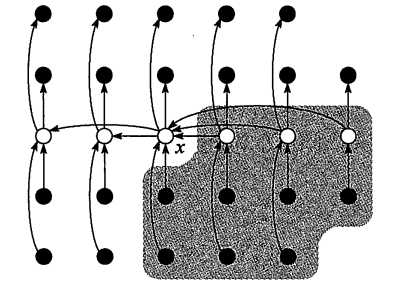
\includegraphics[width=8cm]{fig2}
	\caption{$A[m]$的选取}
	\label{fig2}
\end{figure}

我们考查上述选取方法,如\cref{fig2}所示,首先确定大于$A[m]$的元素个数:

大于$A[m]$的元素应当至少包含$A[m]$所在组的,比$A[m]$大的\textbf{2个}元素,以及中位数大于$A[m]$的组的\textbf{中位数元素}以及\textbf{大于中位数的2个元素},如\cref{fig2}中的阴影区域所示,因此,大于$A[m]$的元素个数$N$可估算为:
$$
N\geqslant 3\left(\left\lceil\frac{1}{2}\left\lceil\frac{n}{5}\right\rceil\right\rceil-2\right)\footnote{$-2$是减去$A[m]$所在的组以及元素数可能不足5个的最后一组}\geqslant\frac{3n}{10}-6
$$

类似可知,至少有$3n/10-6$个元素小于$A[m]$,这也就意味着$A_L,~A_R$的元素个数均为规模$n$的常数因子倍,进而无论剪去哪一个子集,都会剪去常数因子个数据。

以上,我们说明了利用对$A[m]$进行适当的选取,可实现对常数因子个数据的剪枝,以下,我们将分析整个算法的时间复杂度:

我们记算法的时间复杂度为$T(n)$,首先,\textbf{$A[m]$的选取是算法的每一次递归调用都需要进行的},选取步骤的1、2消耗时间复杂度为$O(n)$,选取步骤的3(即寻找$m_i$的中位数)事实上也可以调用原算法解决(因为寻找中位数也是一种选择问题),时间复杂度为$T(\lceil n/5\rceil)$。

其次,对算法的剪枝搜索过程,对$A_L,~A_M,~A_R$的划分消耗$O(n)$的时间复杂度,另外,由于我们证明了$A_L,~A_R$的元素个数均不小于$3n/10-6$,因此在递归时,有$7n/10+6$规模的元素参与下一轮递归,进而我们可得出时间复杂度的递推公式:
$$
T(n)=T\left(\left\lceil\frac{n}{5}\right\rceil\right)+T\left(\frac{7n}{10}+6\right)+O(n)
$$

我们可以通过数学归纳法证明$T(n)=O(n)$,具体证明过程此处不再给出,假设$T(n)\leqslant cn$并进行归纳即可。
	%\blinddocument
\end{document}
